% =============================================================================
%  Supplementary Section S4: Measurement routes at 5% of normal.
%  Order: setting; why the level does not split (arithmetic, Supplementary
%  Fig. sfig:s4amplify); every route in one table (stab:s4routes); measuring
%  the other exit; reading the enzyme directly (stab:s4mapping); why there is
%  no third kind of route (stab:s4carn); the saturable-clearance model
%  (stab:s4sat, stab:s4tight, Supplementary Fig. sfig:s4cond).
% =============================================================================
\section{Measurement routes at 5\% of normal}
\label{si:s4}

This section asks whether any measurement that could be added to the routine record
identifies the residual capacity $\theta$ of a patient with severe propionic acidaemia (PA),
taken throughout as 5\% of normal. It explains why the record alone fails
(Section~\ref{si:s4:split}), collects every route we priced in one table
(Section~\ref{si:s4:table}), discusses measurements of the non-enzymatic route and of the load
(Section~\ref{si:s4:other}) and direct readings of the enzyme (Section~\ref{si:s4:direct}),
sets out why we found no third kind of route (Section~\ref{si:s4:third}), and repeats the
analysis in the saturable-clearance model (Section~\ref{si:s4:sat}). A change in capacity
within one patient escapes these limits; it is the subject of
Supplementary Section~\ref{si:s5}.

% -----------------------------------------------------------------------------
\subsection{Setting}
\label{si:s4:setting}

Unless stated otherwise, every number in this section is computed in the linear-clearance
model (Supplementary Section~\ref{si:s1-eq}). The marker $m$ is plasma 3-hydroxypropionate.
It is cleared by the enzyme, the patient's own capacity $\theta$ plus the increment
$\Delta(t)$ delivered by the infusions, each acting through the saturation
$g(m)=m/(K_m+m)$, and by a non-enzymatic route $k_e m$. The constants are the half-saturation
$K_m=100$\uM, the rate constant $k_e=5$\,d$^{-1}$ and a recorded load $L=323$\um, on a scale on
which normal capacity is 3000\um; 5\% of normal is $\theta=150$\um. The unrecorded load enters
the fits as an offset $b$ on the recorded load.
% src: src/common/models.py:68-74 (ParamsA theta 3000, Km 100, ke 5); manuscript/main.tex:631-634,659; pi_note/pi_note.tex:126-131

The record is the monthly design of the main text: 25 draws over two years on the
fortnightly dose train (a jump $D=6000$\um\ at each infusion and a half-life of 3.5\,d, both
assumed design values), with intake varying by 10\% from day to day and recorded with a 5\%
error, and a 5\% assay coefficient of variation. The prior on $k_e$ is log-normal with a standard deviation of
0.8 on the log scale (a factor of 2.2), the prior on $b$ has a standard deviation of 5\% of
the load, and no prior is placed on $\theta$ or $K_m$. Precision is the Cram\'er--Rao bound on
$\sdl{\hat\theta}$, the standard deviation of the logarithm of the estimate, as a median over
24 simulated intake records, against the target of 0.20.
% src: pi_note/pi_note.tex:129-135; manuscript/main.tex:603-604,684-694,701-702

At 5\% of normal these bounds are optimistic. Given $K_m$ and $k_e$, the likelihood is close
to Gaussian in $\theta$ rather than in $\ln\theta$, so it extends to $\theta=0$ and the profile
likelihood has no lower end (main text, Fig.~3c). We use the bounds to rank routes and to say
which reach the target; where a route comes close to it, a simulated value is given as well.
% src: pi_note/pi_note.tex:135-139; audit/brief_2026-10-01/REPORT.md:151

% -----------------------------------------------------------------------------
\subsection{Why the level does not split: the arithmetic of a shared balance}
\label{si:s4:split}

Consider first a patient at 5\% of normal without therapy, at steady state, so that everything
that comes in also leaves. The load of 323\um\ settles the marker at 54.0\uM. At that level the
enzyme removes 53\um, a share $s=\theta g(m)/L=0.163$ of the load, and the non-enzymatic route
removes 270\um, the other 84\%. A blood draw measures the level; with the load known, the
total removed follows, but not how it is split between the two exits. The
enzyme's part is what is left when the other route's part is subtracted from the total. A
1\% error in the other route's 270\um\ is 2.7\um, which is 5\% of the enzyme's 53\um. In
general, a relative error in the non-enzymatic flux reaches $\theta$ multiplied by
$(1-s)/s=5.1$, and a relative error in the load is multiplied by $1/s$, the ratio of total
clearance to enzymatic clearance (Supplementary Fig.~\ref{sfig:s4amplify}).
% src: audit/brief_2026-10-01/pi_note/figure_guide.tex:218-238 (323, 54, 53 (16%), 270 (84%), 2.7 = 5% of 53); out/t1_identifiability.txt:25 (s 0.163, (1-s)/s 5.134); src/model_A/run.py:387-428 (amplification C(m)/theta g(m))

\begin{figure}[tbp]
\centering
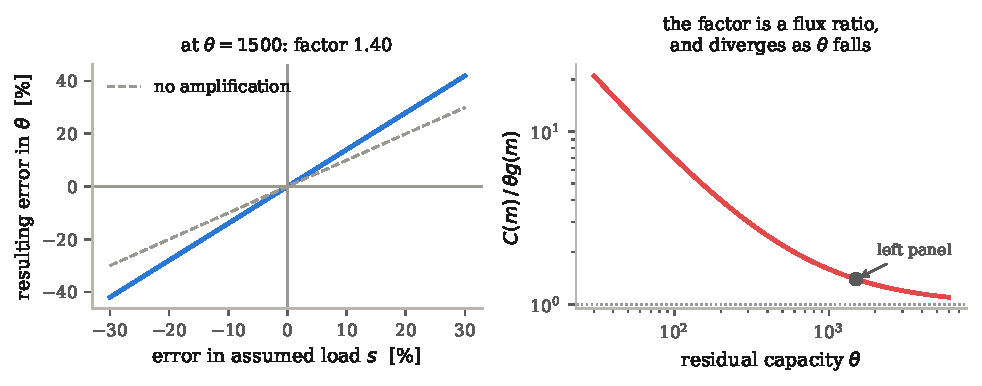
\includegraphics[width=\linewidth]{fig_A5_load_error.pdf}
\caption{\label{sfig:s4amplify}Why an error is amplified when the enzyme's flux is found by
subtraction. Linear-clearance model without therapy, $K_m=100$\uM, $k_e=5$\,d$^{-1}$, with the
marker held at 20\uM. (a)~Relative error in $\hat\theta$ (vertical, \%) produced by a relative
error in the assumed load (horizontal, \%; the load is labelled $s$ in the figure) for a
patient at half of normal capacity, $\theta=1500$\um. The solid line has slope 1.40, against
the dashed line of no amplification. (b)~The amplification factor $C(m)/\theta g(m)$, the total
clearance $C(m)=\theta g(m)+k_em$ divided by the enzyme's flux, against residual capacity
$\theta$ (\um), both axes logarithmic, at the same marker level; the dot marks the case of
panel~a and the dotted line a factor of 1. At this fixed level the factor is
$1+k_e(K_m+m)/\theta$. At steady state the total clearance equals the load, so the factor is
the inverse of the enzyme's share of the load; it grows without bound as $\theta$ falls,
and the amplification is therefore largest in the most severely affected patients.}
\end{figure}
% src: src/model_A/run.py:387-428 (theta 1500, m 20, slope = load_error_factor, ths 30-6000, amp = C/(theta g)); paper/sections/10_results.tex:28-42 (caption: factor 1.4, diverges as theta -> 0)

Supplementary Table~\ref{stab:s4split} lists pairs $(\theta,k_e)$ that produce the same level
from the same load. Any capacity from zero to twice the true value is matched by moving $k_e$
by about 20\% either way. No measurement of $k_e$ in patients exists, and the prior used
throughout allows departures of about a factor of two.
% src: audit/brief_2026-10-01/pi_note/figure_guide.tex:224-238

\begin{table}[htbp]
\centering\small
\caption{\label{stab:s4split}Pairs of residual capacity $\theta$ and non-enzymatic rate
constant $k_e$ that give the same steady-state marker level (54.0\uM) from the same load
(323\um), for an untreated patient whose true capacity is 5\% of normal (150\um) in the
linear-clearance model. Each column explains a settled draw equally well.}
\begin{tabular}{@{}lccccc@{}}
\toprule
capacity $\theta$ (\um) & 0 & 75 & 150 (true) & 300 & 450 \\
$k_e$ giving the same level (d$^{-1}$) & 5.97 & 5.49 & 5.00 & 4.03 & 3.05 \\
change in $k_e$ & $+19\%$ & $+10\%$ & -- & $-19\%$ & $-39\%$ \\
\bottomrule
\end{tabular}
\end{table}
% src: audit/brief_2026-10-01/pi_note/figure_guide.tex:224-230

On therapy the comparison is less favourable still. The delivered enzyme removes most of the
load, so the patient's own enzyme carries only about 6\% of it, and over the levels a treated
patient visits on the monthly record (about 4--38\uM, well below $K_m$) the enzyme's
saturation curve is close to a straight line, which the non-enzymatic route's straight line
can reproduce. On the noiseless profile
likelihood of the monthly record, removing the patient's enzyme altogether raises $k_e$ from
5.0 to 6.1\,d$^{-1}$ and costs the fit almost nothing (Supplementary
Section~\ref{si:s1-pencil}).
% src: audit/brief_2026-10-01/pi_note/figure_guide.tex:272-281 (about 6% on therapy, 16% untreated; k_e 5.0 -> 6.1); pi_note/pi_note.tex:181 and out/t51_pencil_geometry.txt:6 (monthly record m 4.3-37.8); out/t1_identifiability.txt:59 (k_e on the profile 6.108 at 0.01 x truth)

In the Fisher information of the monthly record the same arithmetic appears as a correlation
of $-0.99$ between $\ln\hat\theta$ and $\ln\hat k_e$. The regression of $\ln\hat\theta$ on
$\ln\hat k_e$ has slope $-4.44$, against $-(1-s)/s=-5.13$ in the untreated arithmetic, and
uncertainty in $k_e$ accounts for 98\% of the variance of $\ln\hat\theta$. Knowing $k_e$ exactly
would bring $\sdl{\hat\theta}$ from 3.07 to 0.39, whereas knowing $K_m$ exactly gives 2.89 and
knowing $b$ exactly 3.05. The non-enzymatic route is therefore the binding unknown at this
capacity; the load offset and the half-saturation constant matter little.
% src: out/t1_identifiability.txt:25 (corr -0.9919, beta -4.444, (1-s)/s 5.134, sd 3.0673, |ke 0.3879, |Km 2.8851, |b 3.0463, ke share of var 98.4%)

% -----------------------------------------------------------------------------
\subsection{Every route in one table}
\label{si:s4:table}

Supplementary Table~\ref{stab:s4routes} collects every route to the absolute value of $\theta$
at 5\% of normal that we priced. Routes in the upper part infer $\theta$ through the balance,
from the record alone or with measurements of the non-enzymatic route and of the load. Routes
in the lower part read the enzyme directly. Each precision assumed for a new measurement is
stated in the table. Two routes reach 0.20, both direct readings of the enzyme, and each does
so only if a calibration constant is supplied that has not been measured in humans.
% src: audit/brief_2026-10-01/REPORT.md:13-19,42-50; pi_note/pi_note.tex:216-237

The record alone gives 3.07 when all draws share one pooled noise level, the noise model of
the main analysis (Supplementary Section~\ref{si:s2:setting}), and 3.05 when each draw carries
its own noise level, set by that draw's marker level and recorded load. The route calculations
use the second model, so their reference value is 3.05; the two differ only in how the noise is
modelled (Supplementary Section~\ref{si:s8-how}).
% src: out/t1_identifiability.txt:19 (per-draw ln-m noise instead of n4's single sigma: 5% -> 3.0454); out/t26_multiobservable.txt:5 (3.045); pi_note/pi_note.tex:243-245

\begin{table}[htbp]
\centering\small\setlength{\tabcolsep}{4pt}\renewcommand{\arraystretch}{1.12}
\caption{\label{stab:s4routes}Every route to absolute residual capacity at 5\% of normal, in the
linear-clearance model, added to the monthly record (25 draws over two years on therapy).
Precision is $\sdl{\hat\theta}$, the Cram\'er--Rao bound with each draw at its own noise level,
except where marked. $Y$, precision of a direct reading; $Z$, uncertainty of its calibration
(standard deviation on the log scale); $\kappa$, scale from PCC activity measured in cells to
whole-body capacity; $c$, recovery of a flux reading. Last column: what the route needs that has
not been measured in humans; a dash means that the route needs nothing further but misses the
target.}
\begin{tabular}{@{}>{\raggedright\arraybackslash}p{0.27\linewidth}>{\raggedright\arraybackslash}p{0.18\linewidth}>{\raggedright\arraybackslash}p{0.17\linewidth}>{\raggedright\arraybackslash}p{0.16\linewidth}>{\raggedright\arraybackslash}p{0.14\linewidth}@{}}
\toprule
route & what it reads & assumed precision & $\sdl{\hat\theta}$ & unmeasured constant needed \\
\midrule
\multicolumn{5}{@{}l}{\emph{Inference through the balance}}\\
\addlinespace[2pt]
record alone & marker level & 5\% assay, 5\% load record & 3.05 (3.07 with a pooled noise level) & -- \\
$+$ isotope-dilution load turnover & total appearance rate $L+b$ & 10\% & 3.04 & -- \\
$+$ intravenous $^{13}$C$_3$ tracer & total clearance, hence $k_e$ & 5.4\% & 0.45 & -- \\
$+$ both & & & 0.44 & -- \\
$k_e$ exact (idealised) & & exact & 0.38 & not an instrument \\
$k_e$ and unrecorded load exact (idealised) & & exact & 0.29 & not an instrument \\
as above, per-draw load-record error also removed (idealised) & & exact & 0.19--0.20 (by noise model); simulated 0.215--0.218 & not an instrument \\
\addlinespace
\multicolumn{5}{@{}l}{\emph{Direct readings of the enzyme}}\\
\addlinespace[2pt]
ex vivo PCC assay, $\kappa$ known & activity, $\kappa\theta$ & 20\% repeatability & 0.20 (0.25 at 25\%) & $\kappa$ \\
ex vivo assay $+$ both tracers, $\kappa$ known & & as above & 0.18 & $\kappa$ \\
ex vivo assay, $\kappa$ unknown & & 20\% & 3.05 & -- \\
ex vivo ratio to healthy controls, read as in vitro activity & activity relative to controls & patient 10\%, 30--100 controls & 0.10--0.16 & answers a different question \\
ex vivo ratio, read as whole-body $\theta$ & as above, with per-patient mapping error & $R^2=0.33$, spread 0.6--1.0 log units & 0.65 (0.50--0.80) & mapping with $R^2\ge0.89$--0.96 \\
calibrated in vivo flux reading & flux $c\,\theta g(m)$ & $Y$, $Z$ & 0.20 if $\sqrt{Y^2+Z^2}\le19.3\%$ (18.4\% simulated) & $c$ \\
1-$^{13}$C-propionate breath test as available & fraction oxidised, times $c$ & $c$ not calibrated per patient & no gain from one reading & $c$ \\
\bottomrule
\end{tabular}
\end{table}
% src: out/t26_multiobservable.txt:5-19 (3.045, 0.200, 0.454, 0.384, 3.041, 0.441, 0.291, 0.183, 0.182); out/t1_identifiability.txt:19 (3.07 vs 3.05); REPORT.md:161 (0.204; MC 0.215-0.218); pi_note/pi_note.tex:221-224 (0.19-0.20 CRB depending on the noise model; 0.215-0.218 simulated); out/t27_exvivo_kappa.txt:13,17 (0.200, 0.249, 3.045); out/t28_ratio_route.txt:23-27 (patient 10%: 0.104-0.162 at N = 30-100; REPORT.md:34,709 quote 0.11-0.19, which needs N = 10 at the upper end); out/t29_mapping_scatter.txt:18 (0.503/0.654/0.802), :76-80 (R^2 needed 0.889-0.960); out/t16_flux_observable.txt:13-15 (19.3% / 18.4%); out/t26_multiobservable.txt:24-28 (breath recovery free)

% -----------------------------------------------------------------------------
\subsection{Measuring the non-enzymatic route and the load}
\label{si:s4:other}

\paragraph{The intravenous tracer.} A micro-dose of $^{13}$C$_3$-3-hydroxypropionate, the
labelled marker, given intravenously disappears at the total clearance at the prevailing level $m_0$,
$k_e+\theta/(K_m+m_0)$, from which $k_e$ follows. We took its precision on $k_e$ as 5.4\%.
That value is optimistic, because turning a measured clearance of 3-hydroxypropionate into the
model's $k_e$ needs further assumptions about the overflow pathway that the calculation treats as
exact. At 5.4\% the tracer brings the record from 3.05 to 0.45; even with $k_e$ known exactly
the record gives 0.38.
% src: REPORT.md:668 (IV 13C3-3-HP micro-dose; CL_total = k_e + theta/(K_m+m0); 5.4%, closure assumed free); out/t26_multiobservable.txt:10-11 (0.454, 0.384)

\paragraph{The load.} Whole-body propionate turnover measured by isotope dilution gives the
total appearance rate, $L+b$. At an assumed 10\% precision it is looser than the record's own
5\% prior on $b$, and it leaves the record at 3.04. Together with the tracer it gives 0.44, the
best value among the measurements of the non-enzymatic route and of the load, still more than
twice the target. The estimate is limited by $k_e$, and measuring the load barely changes it.
% src: out/t26_multiobservable.txt:12,16,30-35 (3.041, 0.441; turnover looser than the 5% prior); REPORT.md:52

\paragraph{The idealised limit.} Exact knowledge of $k_e$ and of the unrecorded load is not an
instrument, but it bounds what this family of routes can achieve: 0.29. What remains is the
per-draw error of the load record and of the assay. Removing the load-record error as well
brings the bound to 0.19--0.20, depending on the noise model, and simulated fits give
0.215--0.218 (95\% interval 0.192--0.240), so even this case reaches the target without falling
reliably below it. With $k_e$ exact and the load as recorded, a residual of 0.39 remains at 25
draws with one pooled noise level (0.38 with each draw at its own), of which the load record
contributes 62\% and the assay 29\%. It falls with the number of draws, more slowly than
$1/\sqrt n$ at first because the record constrains the load offset only gradually, and crosses
0.20 near 300 draws, about three a week for two years.
% src: out/t26_multiobservable.txt:17 (0.291); REPORT.md:161 (0.204, MC 0.215-0.218), :249; out/t11_fim_check.txt:243 (MC RMSE 0.2154, 95% [0.1922, 0.2402]); pi_note/pi_note.tex:148-151,221-224 (0.39, 62%, 29%, ~300 draws; 0.19-0.20); REPORT.md:191 (0.39 split 62% load record, 29% assay, t8, pooled noise); out/t1_identifiability.txt:25 (|ke 0.3879 pooled); out/t26_multiobservable.txt:11 (0.384 per-draw)

\paragraph{Other ways to learn $k_e$.} A deliberate 25\% reduction of intake estimates $k_e$
to a standard deviation of about 0.2 on the log scale if the unrecorded load is known to 5\%
and stays constant through the reduction. That assumption may fail in PA, where a cut in intake
can provoke catabolism and raise the load. At that precision no sampling rate, up to two draws a
day for two years, reaches even 0.30. With the unrecorded load known to 1\% the same step would
give $k_e$ to 0.06, and over two years $\sdl{\hat\theta}$ would then be 0.47 with monthly draws,
0.38 with weekly draws and 0.31 with daily draws.
% src: pi_note/pi_note.tex:152-156; out/t26_multiobservable.txt:36-38 (0.285 at 10%, 0.205 at 5%, 0.062 at 1%); out/t22_longitudinal.txt:5-15 (0.465, 0.383, 0.310)

\paragraph{Deliberate perturbations and pooling.} Short, densely sampled experiments outside the
routine record were also examined, over 5280 designs (sampling every 5--60 minutes for 24--72
hours, assay coefficient of variation 0.5--5\%, a range of excursions). At the clinical 5\%
assay no design that adds no propiogenic substrate reaches 0.20, even by the Cram\'er--Rao bound.
At a research-grade 0.5\% assay, an extra dose of the therapy raising the delivered increment to
a peak of 1500\um, sampled every 5 minutes for 72 hours (865 samples) with the delivered
increment known exactly, gives 0.124 (0.131 in simulated fits), and withdrawing half the diet with
the unrecorded load known to 1\% gives 0.195 (0.199 simulated, straddling the target). Raising
the load instead reaches the target at the clinical assay by the Cram\'er--Rao bound
(0.193--0.199 for two- to fourfold loads; simulated fits give 0.217 at a twofold and 0.211 at a
threefold load, missing or straddling it), but every such load lies beyond the carnitine model's
tipping point, which a patient at 10\% of normal crosses at 1.18 times the baseline load, so
these experiments are not admissible. Pooling does not help either: 24 patients at 5\% of normal
who share one value of $k_e$ give 1.17, and 1.82 if $k_e$ varies between them with a standard
deviation of 0.33 on the log scale.
% src: REPORT.md:317-364 (F3: 5280 designs; none without added substrate at 5% CV; drug 1500 N=865 0.124, MC 0.131; withdrawal 50% L0 to 1% 0.195, MC 0.199; load x2-x4 0.193-0.199; fold 1.177), :157-181 (scenario table; load x2 MC 0.217 fails, x3 MC 0.211 straddles), :274-285 (F2: 1.17 at omega 0, 1.82 at 0.33)

% -----------------------------------------------------------------------------
\subsection{Reading the enzyme directly}
\label{si:s4:direct}

\paragraph{Ex vivo assay of PCC activity.} An assay of PCC activity in the patient's cells
reads $A=\kappa\,\theta\,e^{\varepsilon}$, where $\varepsilon$ is the assay's scatter, with a
repeatability $Y$ that we assumed to be 20\%, and $\kappa$ is the scale from activity in cells
to whole-body capacity. With $\kappa$ known, the assay sets the precision on its own: 0.20 at
20\% repeatability, on the target, and 0.25 and 0.30 at 25\% and 30\%. Adding both tracer
measurements gives 0.18. With $\kappa$ uncertain by $Z=\operatorname{sd}(\ln\kappa)$ the
precision follows $\sqrt{Y^2+Z^2}$. At 20\% repeatability no uncertainty in $\kappa$ can be
tolerated, and at 10\% repeatability $\kappa$ must be known to 0.173 on the log scale. No human
study reports $\kappa$. Patients with no capacity of their own cannot calibrate it, since their
activity is zero whatever $\kappa$ is, and we know of no other source of independently known
capacity. With $\kappa$ unknown the assay adds nothing to the record (3.05).
% src: out/t27_exvivo_kappa.txt:5-9 (20% is repeatability; kappa unreported), :11-17 (0.200, 0.249, 0.299; free 3.045), :28-36 (hypot contour; 0.173 at 10%; none at 20%); out/t26_multiobservable.txt:19 (0.182); REPORT.md:687-698 (kappa; theta = 0 carries no kappa information; the repository identifies no source of known nonzero theta); out/t27_exvivo_kappa.txt:101-115

\paragraph{Ratio to healthy controls.} Expressing the patient's activity as a ratio to the mean
activity of healthy controls removes $\kappa$, because it multiplies patient and controls alike.
The precision is then set by the patient's reading and by the error of the control mean,
$\sqrt{Y^2/n_r+\sigma_h^2/N}$ for $n_r$ readings of the patient and $N$ controls with
between-control spread $\sigma_h$. No value of $\sigma_h$ for PCC activity is available, so it
was varied from 30 to 70\%. With the patient read to 10\% and 30--100 controls this gives
0.10--0.16 (0.14--0.24 with 10 controls). That number, however, answers a different question.
It is the precision of in vitro residual activity as a fraction of control, whereas $\theta$ in our model is a whole-body flux
capacity.
% src: out/t28_ratio_route.txt:5-13 (kappa cancels; sigma_healthy has no figure), :23-27 (patient 10%: N = 30-100 0.104-0.162; N = 10 0.138-0.242); REPORT.md:699-709 (hypot(Y/sqrt(reads), sigma_h/sqrt N)); REPORT.md:34,709 and t28:30 round this to 0.11-0.19, whose upper end needs N = 10

\paragraph{Read as whole-body capacity.} Used as an estimate of $\theta$, the ratio carries a
per-patient error that no ratio removes. Write
$\ln(\text{in vitro activity})=a+b_1\ln\theta+\eta$, where $a$ and $b_1$ describe the population
relation and $\eta$ is each patient's departure from it. The departure has standard deviation
$\sigma_\eta=\sqrt{1-R^2}\,s_\theta$, with $R^2$ the share of the between-patient variance of
$\ln\theta$ that the in vitro reading explains and $s_\theta$ the between-patient spread of
$\ln\theta$. The only study that measured both quantities in the same patients, in
methylmalonic acidaemia, found $R^2=0.33$ in 11 patients, with an in vitro incorporation assay
rather than a direct PCC assay, against the in vivo breath test~\cite{breath_test_mma}.
Supplementary Table~\ref{stab:s4mapping} gives the resulting precision. At an assumed spread of
0.8 log units it is 0.65, and 0.50--0.80 over spreads of 0.6--1.0; even $R^2=0.8$ leaves
0.30--0.46. A better control panel does not help once $\eta$ dominates: 0.649 at a control
spread of 16\% against 0.654 at 50\%. Reaching 0.20 would need $R^2$ of 0.89--0.96. A paired
study of direct PCC activity and in vivo propionate oxidation in the same patients with PA would
settle the matter: if the relation is as loose as in methylmalonic acidaemia, 20--30 patients
would bring the upper 95\% bound on $R^2$ down to about 0.60--0.65, well below what the route
needs.
% src: out/t29_mapping_scatter.txt:13-20 (sigma_eta = sqrt(1-R^2) sd_between; table), :31-39 (control spread 16%: 0.649-0.650; 50%: 0.654), :76-80 (R^2 0.889, 0.938, 0.960), :87-91 (N=20: 0.65, N=30: 0.60); REPORT.md:711 (Manoli 2021, MMA, 14C incorporation, not a direct PCC assay, R^2 = 0.327, n = 11)

\begin{table}[htbp]
\centering\small
\caption{\label{stab:s4mapping}Precision $\sdl{\hat\theta}$ of the ex vivo ratio route at 5\% of
normal when the ratio is read as whole-body capacity, against the share $R^2$ of
between-patient variance that the in vitro reading explains and the between-patient spread of
$\ln\theta$ (assumed). The patient is read to 10\%, with 30 healthy controls and a 50\%
between-control spread; the record contributes negligibly. $R^2=0.33$ is the value measured in
methylmalonic acidaemia~\cite{breath_test_mma}; 0.5 and 0.8 are optimistic. The last row gives
the $R^2$ at which the route would reach 0.20.}
\begin{tabular}{@{}lccc@{}}
\toprule
& \multicolumn{3}{c}{between-patient spread of $\ln\theta$} \\
\cmidrule(l){2-4}
& 0.6 & 0.8 & 1.0 \\
\midrule
$R^2=0.33$ (measured, methylmalonic acidaemia) & 0.503 & 0.654 & 0.802 \\
$R^2=0.5$ & 0.441 & 0.571 & 0.701 \\
$R^2=0.8$ & 0.299 & 0.380 & 0.462 \\
\addlinespace
$R^2$ needed for 0.20 & 0.889 & 0.938 & 0.960 \\
\bottomrule
\end{tabular}
\end{table}
% src: out/t29_mapping_scatter.txt:16-20,76-80

\paragraph{A calibrated in vivo flux reading.} A reading proportional to the enzymatic flux in
vivo, $O=c\,\theta g(m)$ with recovery $c$, would avoid both problems if $c$ were known. With
$Y$ the precision of the reading and $Z$ the uncertainty of $c$ on the log scale, the Fisher
information is exactly that of one calibrated reading of precision $\sqrt{Y^2+Z^2}$. The target
is met when $\sqrt{Y^2+Z^2}\le19.3\%$ by the Cram\'er--Rao bound, or 18.4\% in 2000 simulated fits
per point (90\% bootstrap interval 17.9--19.0\%). With $c$ known to 10\% the simulated threshold
on $Y$ falls to 16.0\%. Averaging $n$ readings divides $Y$ by $\sqrt n$ but leaves $Z$, so the
calibration sets a floor that repetition does not lower. The threshold is nearly the same at
every capacity from 1 to 20\% of normal (19.3--19.5\%). Writing the reading instead as the
fraction of the load that is oxidised, $S=\theta g(m)/L$, together with a measurement of the
load, moves the calibration onto the load measurement and leaves the requirement unchanged: the
pair reaches the target at $S$ to 19.7\% with the load exact and 19.6\% with the load known to
5\%.
% src: out/t16_flux_observable.txt:5-21 (hypot collapse, 19.33% FIM, 18.4% MC; averaging divides Y not Z), :23-39 (s and L on the same locus: 19.69%, 19.60%); REPORT.md:175-177 (18.4% [17.9, 19.0], 90% bootstrap; recovery to 10%: 16.0%), :155 (intervals 90% unless marked); out/t21_sensitivity.txt:35-42 (19.4, 19.4, 19.3, 19.3, 19.5% at 1-20%)

\paragraph{The breath test.} The 1-$^{13}$C-propionate breath test reads the fraction of a
labelled dose that is oxidised, multiplied by a recovery that is not calibrated for each
patient. With that recovery unknown, one reading adds nothing to the record; carried as an
unknown shared by several readings, about 70 readings at a 5\% reading precision would be
needed at 10\% of normal, and more at 5\%. Its only published repeatability, between visits in
methylmalonic acidaemia (6.9\% in controls)~\cite{breath_test_mma}, is given for patients in
Supplementary Section~\ref{si:s2:record}. We found no instrument available today that meets the
specification of a calibrated flux reading.
% src: out/t16_flux_observable.txt:41-51 (breath reads s with unknown recovery c; one reading worthless); out/t26_multiobservable.txt:24-28 (~70 readings at 10% capacity, more at 5%); paper/claims.csv:44 (6.9% controls; 14.0%, 0.4-50.8%, n=15); REPORT.md:32 (no human instrument for the flux specification)

% -----------------------------------------------------------------------------
\subsection{Why we found no third kind of route}
\label{si:s4:third}

In the model the patient's enzyme acts only through the flux it carries, $\theta g(m)$, of which
$\theta$ is the maximal value. An observable can therefore depend on $\theta$ in one of two ways.
It can depend on the states that this flux helps to set, such as the marker level; inverting the
balance then requires the shape of the competing non-enzymatic route ($k_e$ in the
linear-clearance model; its maximal rate $V_e$ and half-saturation $K_e$ in the
saturable-clearance model; $K_c$, $M_i$, $\rho_0$ and $R_0$ in the carnitine model). Or it can
read the flux itself, scaled by a transduction constant ($\kappa$ for the ex vivo assay, the
recovery $c$ for a breath test), which must then be known. A marker of an upstream pool, such as
propionylcarnitine or 2-methylcitrate, would need both a calibration and the balance of that
pool. Such markers cannot be priced in our model, which has no propionyl-CoA state, and five of
the ten candidate observables we listed were set aside for that reason (the breath test among
them, which we priced above only in a simplified form); each of the other five falls on one side
or the other.
% src: REPORT.md:23-28 (two kinds; no third; upstream pool needs both; ten-sensor panel), :657-668 (ten candidates, five dropped for want of a propionyl-CoA state); pi_note/pi_note.tex:252-258; figure_guide.tex:64-79

The same conclusion follows from the physiology without the model. At steady state the net
carboxylation flux equals the rate at which propiogenic substrate is disposed of, so a
concentration reports the size of a pool set by inflow and outflow rather than the throughput
of one step, and no concentration can isolate the carboxylation step without a tracer.
% src: REPORT.md:32

The carnitine model is the decisive test, because there the competing route has an observable
of its own, free carnitine, whose steady state does not involve $\theta$. A patient at 5\% of
normal has no steady state at the carnitine model's baseline load of 600\um, so we evaluated it
at a managed load of 500\um. Supplementary Table~\ref{stab:s4carn} gives the result. With the
route's constants known, the marker alone reaches 0.34, and free carnitine adds nothing. With the
constants free, free carnitine moves the precision only from 19.9 to 16.3, and to 17.7 once plasma
free carnitine is treated as an unknown fraction of the modelled pool, as it should be, since
plasma holds under 1\% of the body's carnitine. Observing the competing route does not remove
the need to know its shape.
% src: out/t41_model_c.txt:5-19 (load 500; m only free 19.92; m+c free 16.30; known 0.34; one free at a time 0.34-0.49); out/t43_plasma_pool.txt:11-18 (17.70, 17.73; m-only known 0.34), :21-24 (<1% in plasma); REPORT.md:28,810

\begin{table}[htbp]
\centering\small
\caption{\label{stab:s4carn}Precision $\sdl{\hat\theta}$ at 5\% of normal in the carnitine model,
at a managed load of 500\um, when the marker is read with or without plasma free carnitine. Route
constants: the half-saturation of conjugation $K_c$, the level $M_i$ at which acylcarnitine
competition doubles carnitine loss, the relative basal loss $\rho_0$, the replenishment $R_0$
and the conjugation rate $k$. Plasma fraction: free carnitine in plasma as an unknown fraction
of the modelled pool, constant or drifting with the load.}
\begin{tabular}{@{}lc@{}}
\toprule
observables and route constants & $\sdl{\hat\theta}$ \\
\midrule
marker alone, route constants free & 19.9 \\
marker and free carnitine, route constants free & 16.3 \\
\quad plasma fraction free & 17.7 \\
\quad plasma fraction free and drifting with the load & 17.7 \\
marker alone, route constants known & 0.34 \\
marker and free carnitine, route constants known & 0.34 \\
marker and free carnitine, one constant free: $K_c$, $\rho_0$, $M_i$, $R_0$, $k$ & 0.44, 0.36, 0.49, 0.38, 0.34 \\
\bottomrule
\end{tabular}
\end{table}
% src: out/t41_model_c.txt:10-19; out/t43_plasma_pool.txt:11-18

Every constant these routes need ($k_e$, $b$, $K_m$, $\kappa$, $c$, $V_e$, $K_e$) is a property
of the patient, which is why a change in capacity within one patient escapes the obstacle that
blocks its level (Supplementary Section~\ref{si:s5:cancel}).
% src: REPORT.md:30,573

% -----------------------------------------------------------------------------
\subsection{The saturable-clearance model}
\label{si:s4:sat}

The linear-clearance model gives the non-enzymatic route 84\% of the load at 5\% of normal, more
than the urinary output of propionate metabolites measured in PA, a few per cent of estimated
production~\cite{thompson1990fasting}. A route of limited capacity is closer to the disease. We
therefore repeated the analysis with $\alpha(m)=V_em/(K_e+m)$, where $V_e$ is the route's maximal
rate and $K_e$ its half-saturation; the model, its nominal constants and the constructed
operating point used below are defined in Supplementary Section~\ref{si:s1-eq}. Neither
constant has a source or a row in the model's own provenance registry.
% src: manuscript/main.tex:529-531; REPORT.md:774 (Model B unregistered), :804; src/common/models.py:78-83 (ParamsB ke = V_max 400, Ke 300)

\paragraph{At the nominal constants.} With $V_e=400$\um\ and $K_e=300$\uM, the load that
places the marker at 10\uM\ at normal capacity, 285.6\um, lies below $V_e$, so a patient with
no enzyme of their own could be maintained.
Untreated at 5\% of normal the marker settles at 243.7\uM, where the enzyme carries 0.372 of the load, against 0.163
in the linear-clearance model (Supplementary Table~\ref{stab:s4sat}). Because the route
saturates, it cannot absorb a rising marker as the straight line does, and the enzyme keeps a
larger share at every low capacity (0.586 against 0.292 at 10\% of normal, 0.089 against 0.036 at
1\%). The precision improves accordingly: 0.92 with $K_e$ fixed at its true value and 1.04 with
$K_e$ free under a 50\% prior, against 3.05. It is finite because over the dosed record the
marker stays between 4.1 and 58.7\uM, where the route's saturation $m/(K_e+m)$ is still rising
(from 0.013 to 0.164).
% src: out/t33_model_b.txt:10-16 (anchored load 285.6 at V_e 400), :29-37 (shares and m by capacity), :39-45 (3.045, 0.923, 1.041), :47-54 (record m 4.1-58.7; h 0.013-0.164)

The gain comes almost entirely from the enzyme's share. If $\sdl{\hat\theta}$ scales with
$(1-s)/s$, the clearance carried by the uncertain route relative to the enzyme's, a share rising
from 0.163 to 0.372 lowers $(1-s)/s$ from 5.13 to 1.69, a factor of 3.04, which is 92\% of the
observed factor of 3.30. The remainder comes from the extra unknown $K_e$ and the shifted
operating point.
% src: out/t36_reconcile_remark15.txt:5-11

\paragraph{Joint conditioning.} The joint problem is worse conditioned, as the exchange symmetry
of Supplementary Section~\ref{si:s1-si} leads one to expect. For the sensitivities of the total
clearance at normal capacity, the condition number at a 10\% excursion of the marker rises from
$1.1\times10^5$ in the linear-clearance model to $4.8\times10^7$, about 450-fold
(Supplementary Fig.~\ref{sfig:s4cond}). For the column-normalised sensitivities of the monthly
record at 5\% of normal (one row per draw, saturable-clearance model at its nominal constants),
it rises 18-fold, from 90 to $1.6\times10^3$, and the whole increase lies in the $K_e$ column:
with $K_e$ fixed the condition number is 75, no worse than in the linear-clearance model. The
marginal precision on $\theta$ improves even so, because the priors on the non-enzymatic
constants absorb the ill-conditioned directions. Without those priors (the prior on $b$ kept)
and with $K_e$ free, $\sdl{\hat\theta}$ is 55.5 in the saturable-clearance model at its nominal
constants (52.8 at the constructed point below) against 5.9 in the linear-clearance model
without its prior on $k_e$. The statement that the linear-clearance
model is the most favourable case for identification therefore holds for the joint
conditioning, but not for the marginal precision on $\theta$, which follows the enzyme's share.
% src: paper/sections/03_dynamic.tex:352-353 (1.1e5 -> 4.8e7, about 450); out/t36_reconcile_remark15.txt:13-18 (89.77, 1641, 74.60; 18x; cond of the column-normalised flux-row sensitivity matrix, t36_reconcile_remark15.py:26-39), :24-33 (A no k_e prior 5.908; B no priors, Ke free 55.509, ParamsB record, t36_reconcile_remark15.py:38); out/t38_model_dependent.txt:19 (52.82 at V_e 100, L 220); audit/brief_2026-10-01/t33_model_b.py:100-115 (fim_B: b prior always kept); t38_model_dependent.py:52

\begin{figure}[tbp]
\centering
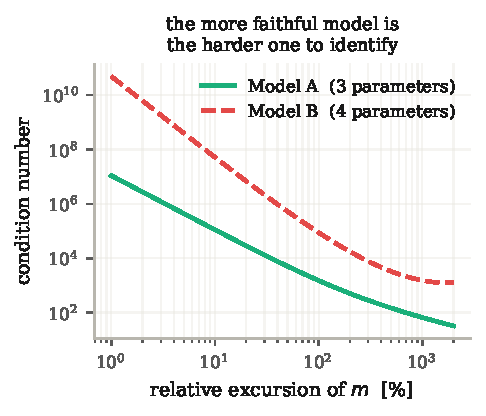
\includegraphics[width=0.6\linewidth]{fig_B4_cost.pdf}
\caption{\label{sfig:s4cond}Joint conditioning of the linear-clearance and saturable-clearance
models at normal capacity. Vertical: condition number of the column-normalised matrix of
sensitivities of the total clearance to the unknowns (logarithmic). Horizontal: relative
excursion of the marker between the levels sampled (\%, logarithmic). The marker is taken at
10\uM\ and at levels raised by one, two and, for the saturable-clearance model, three times the
excursion, one level per unknown, as for a followed trajectory (Supplementary
Section~\ref{si:s1-si}). Solid line, labelled ``Model A (3 parameters)'' in the figure: the
linear-clearance model, unknowns $\theta$, $K_m$ and $k_e$ at $\theta=3000$\um,
$K_m=100$\uM\ and $k_e=5$\,d$^{-1}$. Dashed line, labelled ``Model B (4 parameters)'': the
saturable-clearance model, unknowns $\theta$, $K_m$, $V_e$ and $K_e$ at its nominal constants
$V_e=400$\um\ and $K_e=300$\uM. At a 10\% excursion the condition numbers are $1.1\times10^5$ and
$4.8\times10^7$. The figure shows the cost of a second saturable exit to the joint problem; it
does not show the marginal precision on $\theta$, which improves in the saturable-clearance model
(Supplementary Table~\ref{stab:s4sat}).}
\end{figure}
% src: src/model_B/run.py:142-161 (m0 10, levels m0[1, 1+sp, 1+2sp, 1+3sp], A on 3 levels, B on 4; ParamsA, ParamsB); src/common/models.py:67-83,261-275; paper/sections/10_results.tex:203-219; paper/sections/03_dynamic.tex:352-353

\paragraph{A constructed operating point.} Because the nominal constants do not represent severe
PA, we also use the constructed operating point ($V_e=100$\um, below the untreated load, so that
a patient with no enzyme cannot be maintained; managed load 220\um, at which a patient at 5\%
of normal has a margin of about 1\% of normal). Neither value is measured; both were chosen.
Untreated, this patient would settle at 1272.8\uM, close to where total clearance levels off,
with an enzyme share of 0.632, but over the dosed record the marker stays between 3 and 52\uM.
The precision is 0.29 with $K_e$ fixed and 0.32 with $K_e$ free under a 50\% prior, against 3.05
for the linear-clearance model at the same managed load. Over maximal rates $V_e$ of
50--200\um\ and managed loads of 180--240\um, wherever a steady state exists, it runs from 0.21
to 0.49 (median 0.38), above the target everywhere. It follows $V_e$, which sets the enzyme's
share, and barely depends on the managed load.
% src: out/t35_managed_load.txt:5-17 (V_e 100 below L0 276; L 220: theta_crit 4.0%, margin 1.00%), :41-50 (m 36.1/1272.8; record [3,52]; share 0.632; 3.046, 0.292, 0.317; contrast 0.132, 0.078); out/t38_model_dependent.txt:45-64 (choices; grid 0.21-0.49, median 0.38), :16-18 (0.29, 0.32)

\begin{table}[htbp]
\centering\small\setlength{\tabcolsep}{4pt}
\caption{\label{stab:s4sat}The linear-clearance and saturable-clearance models at 5\% of normal.
Nominal: the saturable-clearance model at $V_e=400$\um, $K_e=300$\uM, with the load that places
the marker at 10\uM\ at normal capacity. Constructed: $V_e=100$\um, below the untreated load,
and a managed load of 220\um. Precision is $\sdl{\hat\theta}$ for the monthly record with the
priors of Section~\ref{si:s4:setting} unless stated; the prior on $V_e$ takes the place of the
prior on $k_e$. ``No prior on the route's constants'' removes the prior on $k_e$ in the
linear-clearance model and those on $V_e$ and $K_e$ in the saturable-clearance model, keeping the
prior on $b$. Within-patient contrast: the Cram\'er--Rao standard deviation of
$\ln\theta_2-\ln\theta_1$ for two windows of 104 draws (Supplementary Section~\ref{si:s5}).}
\begin{tabular}{@{}>{\raggedright\arraybackslash}p{0.40\linewidth}ccc@{}}
\toprule
& linear-clearance & saturable, nominal & saturable, constructed \\
\midrule
load (\um) & 323 & 285.6 & 220 (managed) \\
patient with $\theta=0$ maintainable & yes & yes & no \\
untreated steady-state marker (\textmu M) & 54.0 & 243.7 & 1272.8 \\
enzyme's share of the load at that state & 0.163 & 0.372 & 0.632 \\
$\sdl{\hat\theta}$, $K_e$ fixed & 3.05 & 0.92 & 0.29 \\
$\sdl{\hat\theta}$, $K_e$ free (50\% prior) & -- & 1.04 & 0.32 \\
$\sdl{\hat\theta}$, no prior on the route's constants, $K_e$ free & 5.9 & 55.5 & 52.8 \\
$\sdl{\hat\theta}$, $V_e$ known to 5.4\%, $K_e$ fixed & -- & -- & 0.186 \\
within-patient contrast & 0.133 & 0.088 & 0.078 \\
\bottomrule
\end{tabular}
\end{table}
% src: out/t33_model_b.txt:10-16,29-45,56-58 (285.6; 54.0/243.7; 0.163/0.372; 3.045/0.923/1.041; contrast 0.133/0.088); out/t35_managed_load.txt:41-50 (1272.8, 0.632, 0.292, 0.317, 0.078); out/t36_reconcile_remark15.txt:28-32 (5.908, 55.509); out/t38_model_dependent.txt:19-20 (52.82, 5.86); out/t40_kepoint_robustness.txt:54 (0.186)

\paragraph{What it takes to reach the target.} At the constructed point the target can be
touched only by supplying two unmeasured constants (Supplementary Table~\ref{stab:s4tight}).
With the prior on $V_e$ tightened to 5.4\%, the precision the intravenous tracer provides for
$k_e$ in the linear-clearance model, and $K_e$ fixed, the precision is 0.186. The calculation
grants that precision directly on $V_e$, although in this model the tracer's clearance depends on
both $V_e$ and $K_e$. Across the grid of maximal rates and loads under these conditions it lies
between 0.181 and 0.202, within 0.002 of the target everywhere (at or below it in 10 of 13
cells) and comfortably below it nowhere; with a looser prior of 0.2 on $\ln V_e$ it ranges from
0.183 to 0.228, and only maximal rates up to 100\um\ pass. The
result also needs $K_e$. The precision stays at or below 0.20 only while $K_e$ is known to about
30\% (0.200 at a standard deviation of 0.30 on the log scale, 0.223 at 0.50, 9.3 with $K_e$
free). No measurement of $K_e$ exists, and because the route lumps several processes with
different kinetics, a single half-saturation constant may not exist at all.
% src: out/t38_model_dependent.txt:24-39; out/t40_kepoint_robustness.txt:5-11 (prior 0.2: 0.183-0.228, 5/13), :14-20 (prior 0.054: 0.181-0.202, 10/13), :52-63 (K_e tolerance); REPORT.md:21,796-802; src/common/params.py (no ParamsB row; REPORT.md:774)

\begin{table}[htbp]
\centering\small
\caption{\label{stab:s4tight}Saturable-clearance model at the constructed operating point
($V_e=100$\um, managed load 220\um), 5\% of normal, monthly record: $\sdl{\hat\theta}$ as the
priors on the route's constants are tightened. (a)~Against the prior on $\ln V_e$, with $K_e$
fixed or carrying a prior of 0.3 or 0.1 on $\ln K_e$. (b)~Against the uncertainty of $K_e$, with
the prior on $\ln V_e$ at 0.054 (the 5.4\% of the intravenous tracer). Values at or below the
target of 0.20 are in bold.}
\begin{tabular}{@{}lccc@{}}
\toprule
\multicolumn{4}{@{}l}{(a) prior on $V_e$}\\
\midrule
$\operatorname{sd}(\ln V_e)$ & $K_e$ fixed & $\operatorname{sd}(\ln K_e)=0.3$ & $\operatorname{sd}(\ln K_e)=0.1$ \\
\midrule
0.80 & 0.292 & 0.301 & 0.293 \\
0.40 & 0.217 & 0.229 & 0.219 \\
0.20 & \textbf{0.194} & 0.207 & \textbf{0.195} \\
0.10 & \textbf{0.187} & 0.201 & \textbf{0.189} \\
0.05 & \textbf{0.186} & \textbf{0.200} & \textbf{0.187} \\
\midrule
\multicolumn{4}{@{}l}{(b) uncertainty of $K_e$, $\operatorname{sd}(\ln V_e)=0.054$}\\
\midrule
$\operatorname{sd}(\ln K_e)$ & \multicolumn{3}{c}{$\sdl{\hat\theta}$} \\
\midrule
0 (fixed), 0.05, 0.10 & \multicolumn{3}{c}{\textbf{0.186}, \textbf{0.186}, \textbf{0.187}} \\
0.20, 0.30 & \multicolumn{3}{c}{\textbf{0.192}, \textbf{0.200}} \\
0.50, 1.00 & \multicolumn{3}{c}{0.223, 0.307} \\
free (no prior) & \multicolumn{3}{c}{9.337} \\
\bottomrule
\end{tabular}
\end{table}
% src: out/t38_model_dependent.txt:24-31; out/t40_kepoint_robustness.txt:52-61

The size of the shortfall therefore depends on the clearance structure, from about fifteenfold
in the linear-clearance model to about 1.5-fold at the constructed point of the
saturable-clearance model. In every structure we tested, however, the target is reached only
when a constant that has not been measured in humans is supplied: a calibration for a direct
reading, or the shape of the competing route for an inference through the balance.
% src: out/t38_model_dependent.txt:5-9 (misses by ~15x and ~1.5x); pi_note/pi_note.tex:266-277; out/t40_kepoint_robustness.txt:69-75
